\chapter{DTU Space coating facility}\label{chap:coating_facility}
The multilayer coating facility consists of a vacuum chamber placed in the laboratory known as the Multilab. It started out as a vapor deposition chamber for the SODART mission\cite{Christensen:1997kk,Schnopper:1994ip}. Capable of vaporising a gold wire with a W rod in the center of the chamber, it would deposit a layer of gold on any mirror facing the center. The chamber was later upgraded with magnetron cathodes, each with independent shutters.

The currently used cathodes are attached to powerful DC power supplies that can deposit films atom-by-atom instead of the larger gold particles that would come from vaporisation. The upgrade made it possible to coat multilayers with d-spacings thinner than 3 nm and eventually became the coating method used for the NuSTAR mission.

The entire lab was moved from Rockefeller Institute near Rigshospitalet in Copenhagen during the summer of 2012. It was up and running again around the summer of 2013 in the newly constructed building 328, the new home for DTU Space on DTU campus. In the new location, the lab is 50\% larger, has a double airlock (earlier just a single airlock), laminar airflow from ceiling mounted HEPA filters and various other improvements. The result is a considerably cleaner facility, which is important to avoid contaminants on optical substrates.

\begin{figure}[htbp]
  \centering
  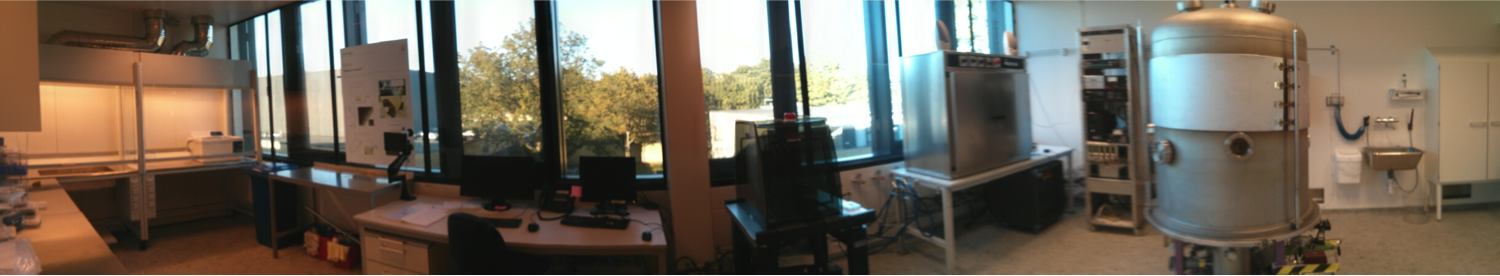
\includegraphics[width=\linewidth]{figures/chamber/multilab1.png}
  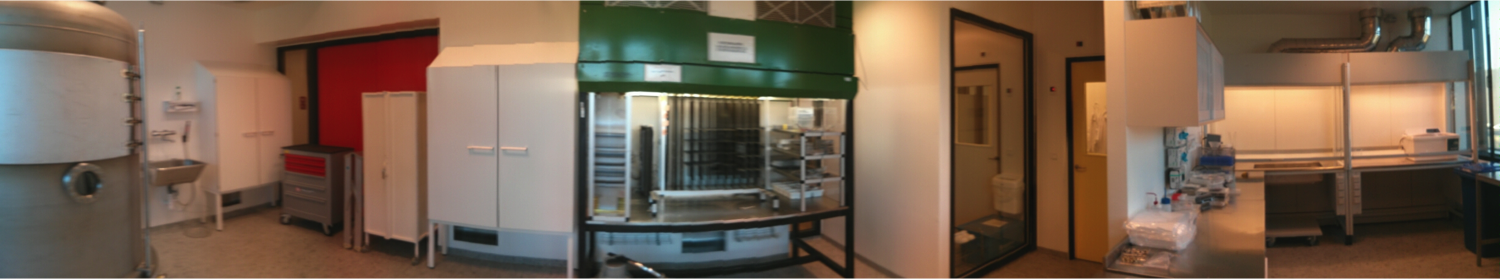
\includegraphics[width=\linewidth]{figures/chamber/multilab2.png}
  \caption{\footnotesize Panoramic view of the Multilab coating facility at DTU Space. Top right can be seen the bell-shaped coating chamber.}
  \label{fig:multilab}
\end{figure}

The vacuum chamber is the dominant piece of the laboratory and most of the computers, electronics and cooling in the lab is in some way connected to the chamber. Apart from the chamber, the lab consists of a downflow module, two fume hoods, a profilometer, a large clean room oven and various tables and cupboards (see figure \ref{fig:multilab}). Next to the lab is the Multilab Auxiliary Room, which houses the cooling heat exchangers and pumps, the rotary vane roughing pump, DC power supplies, and a large part of the extra storage needed for the lab. Additionally, there is a room in the basement that houses a ceramic oven that has a built in vacuum chamber, the room also serves to store hundreds of spare pieces of NuSTAR optic glass.

\section{Coating chamber}
The coating facility at DTU Space is arranged with vertical sputtering cathodes pointing outwards in a circular vacuum chamber, see figure \ref{fig:chamber}. Substrates are mounted on vertical mounting plates that are placed on a rotating ring in the sputtering chamber and the substrates pass in front of each cathode at a speed determined by the desired layer thickness.

\begin{figure}[htbp]
  \centering  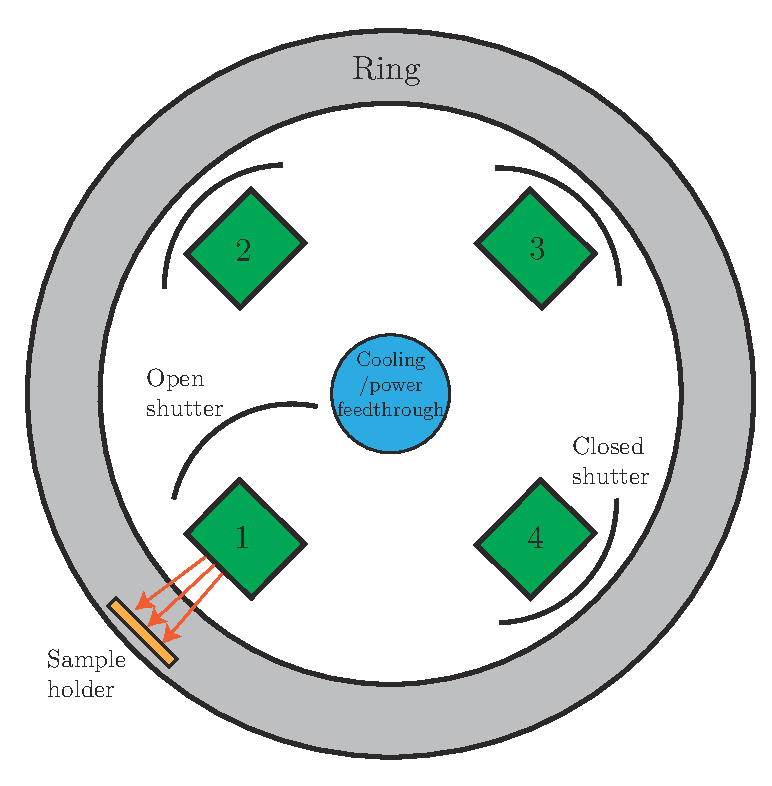
\includegraphics[width=0.5\linewidth]{figures/chamber/chamber.pdf}
  \caption{\footnotesize Diagram of the coating chamber at DTU Space, showing the principle of the rotating sample ring stage. Cathodes 1--4 (green) points outwards and can be covered with a shutter. Water cooling and power lines for the cathodes comes from the floor in the center of the chamber (blue) and connects to the top of each cathode with vacuum flex tubes. The sample (orange) is placed on a vertical plate that is mounted on the ring (grey). The ring rotates, so the samples move past the cathodes and gets coated with a film thickness related to the ring speed.}
  \label{fig:chamber}
\end{figure}

After chamber is closed, a roughing pump and a turbo molecular pumps evacuates the chamber to a pressure of $\leq2\cdot10^{-6}$ Torr before pure Ar gas is let into the chamber at a constant flow rate to ensure the fraction of other gases to be $<$0.1\%. The desired total pressure with Ar gas is $2.8\cdot10^{-3}$ Torr, which is as low as possible while maintaining plasma stability.

The chamber fits four cathodes at a time and the Multilab has six in total, so two can be serviced while the other four are in use. For most coatings, only two or three cathodes at a time are necessary for the same number of materials.

In the earlier software solution, all cathodes were switched on at the same time during deposition of a bilayer. That necessitated two cathodes running with the low-Z material while one cathode ran with the high-Z material in order to achieve the correct $\Gamma$ value and to have each cathode running in a possible power regime. A typical Pt/C  multilayer for NuSTAR required $\Gamma = 0.6$, which meant that 60\% of a material in a bilayer had to be carbon. Platinum and carbon has vastly different coating rates, so one cathode with platinum running at 150 W required two cathodes of carbon running at 900 W in order to achieve $\Gamma = 0.6$. With the new software only one cathode with each kind of material is necessary, but at the expense of a longer coating time.

\subsection{Magnetron cathodes}
The cathodes are the most important part of the chamber. They are 20 inches long and 1/2 inch wide planar magnetron cathodes made by Angstrom Sciences Inc. A diagram of the cathode can be seen in figure \ref{fig:cathodeintersection}. A copper block acts as the cathode with a stainless steel shield around it, separated by teflon spacers. Inside the copper block, three permanent magnets with alternating field directions supplies a magnetic field in front of the cathode. Water cooling and power lines are connected from the cathode through a flexible vacuum tube to water cooling and power supplies outside the chamber. The anode shield is grounded along with the rest of the chamber.

\begin{figure}[htbp]
  \centering  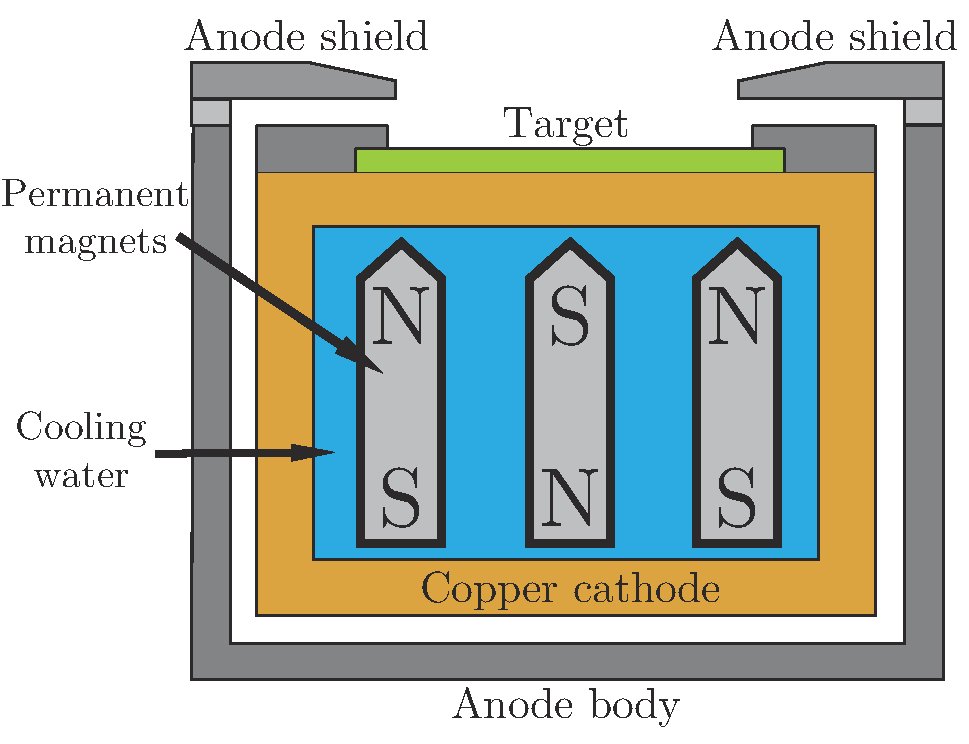
\includegraphics[width=0.5\linewidth]{figures/chamber/cathodeintersection.pdf}
  \caption{\footnotesize Cross-sectional diagram of a magnetron cathode used in the Multilab at DTU Space. }
  \label{fig:cathodeintersection}
\end{figure}

Materials for sputtering, called targets, are fastened to the copper block using a stainless steel clamp. It is important for the target to have a uniform contact with the cathode, so the copper block should be cleaned before fastening using cleanroom wipes and ethanol. For tougher blemishes, a micro-fine sanding sponge can be used to clean the surface followed by ethanol and cleanroom wipes.

Applying a voltage of -400 V to the cathode creates an electric field in front of the target. The argon gas present in the chamber will be ionised in front of the cathode by the electric field, stripping an electron from the argon atoms resulting in a plasma. The positive Ar$^+$ ions are accelerated towards the target, whereby the collision with the target create a sputtering of target atoms in a cone directed normal to the target surface, see figure \ref{fig:sputtering}. A substrate placed opposite the cathode will be coated with the sputtered atoms at a rate proportional to the electric current applied to the cathode.

\begin{figure}[htbp]
  \centering  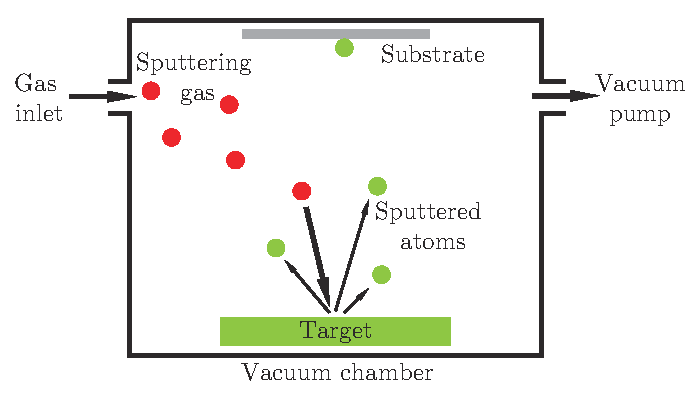
\includegraphics[width=0.6\linewidth]{figures/chamber/sputtering.pdf}
  \caption{\footnotesize Principle of sputtering. Sputter gas led into an evacuated chamber is forced to the surface of a target with a force that rips atoms from the material. The freed target atoms move away from the target and some hit a substrate opposite the target. }
  \label{fig:sputtering}
\end{figure}

Electrons stripped from argon atoms are captured by the magnetic field lines from the permanent magnets in the copper block. The electrons are moved back and forth across the target and occasionally hits neutral argon atoms, which also become ionised and thereby sustain the plasma. The movement of electrons are from the center of the target to the outer edge, and as more argon atoms are ionised in between those two points, the main erosion of the target during coating takes place in a so-called \emph{race track} around the target.
%
% !!!!!Something about the physics of sputtering!!!!!
%
% !!!!Thornton zone model?????!!!!!!

\section{X-ray lab source at DTU Space}
Measurements at DTU Space were done with a reflectivity setup consisting of a rotating copper-anode providing X-ray photons for two beams. One beam is used for reflectivity measurements and the other can be set up for measuring curvature in glass substrates.

After the source, along the z-axis, is placed two slits, a monochromator, an attenuator, on more slit, the sample holder and finally the detector, see figure \ref{fig:xraysetup}. The first two slits ensures that only a narrow beam hits the monochromator, which then reflects only photons around the copper K$_{\alpha_1}$ emission line (8.047 keV) by reflecting the beam on two germanium crystals at an angle where Bragg reflection only allow photons of that energy. The beam continues through the next two slits, thereby minimizing divergence and also filters out a large part of unwanted reflections from the monochromator to ensure a narrow bandwidth. The attenuator ensures that the beam intensity is not too large, thereby saturating the detector.

\begin{figure}[!h]
  \center
  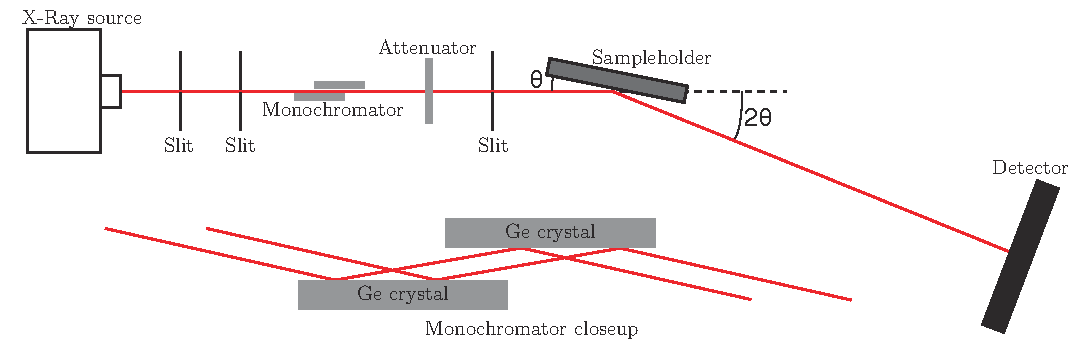
\includegraphics[width=0.8\linewidth]{figures/chamber/xraysetup.pdf}
\caption{\footnotesize Diagram of the X-ray setup at DTU Space. X-ray photons from the source goes through two slits, a monochromator, an attenuator and one more slit before hitting the sample. The reflected photons from the sample travel to the detector which is rotated at a $2\theta$ angle. Below: The monochromator that consists of two germanium crystal that reflect only a given wavelength on the (111) surface using the Bragg principle.}\label{fig:xraysetup}
\end{figure}

The sample holder consists of a slab of flat perforated ceramic material, a vacuum chuck, mounted vertically. It is connected to a pump, which allows flat substrates, like pieces of Si-wafer, to stick very firmly to the stone slab. This method of sample mounting makes it possible to change samples very fast and easy between measurements. The sample holder is centered and mounted on a rotating stage, $\theta$, and can also move in and out of the beam along the x-axis.\\
After the sample holder, 995 mm further along the z-axis is a 10 cm wide 2D methane-gas detector mounted on a rotating stage, $2\theta$. It is centered on the same axis as $\theta$, allowing the detector to move 90\degr around the sample while maintaining a focus on the same spot. The detector has 2000 channels along the x-axis of the beam; 100 channels are used during a measurement, giving a horizontal detector aperture of 2 cm.

\section{Coating calibration}\label{sec:coating_calib}
To deposit a coating with the correct film layer thicknesses on a substrate, a calibration of the material combination is required. Four samples of 10 bilayer films are coated using the two materials. Each sample is placed on a separate mounting plate and each coated with a different thickness of both light and heavy materials. The samples are then measured using XRR and compared to an IMD\cite{Windt:1998tb} model fit to get bilayer thickness (d-spacing) and light/heavy material fraction ($\Gamma$) as seen in figure \ref{fig:irb4c-fit}.

\begin{figure}[!h]
  \center
  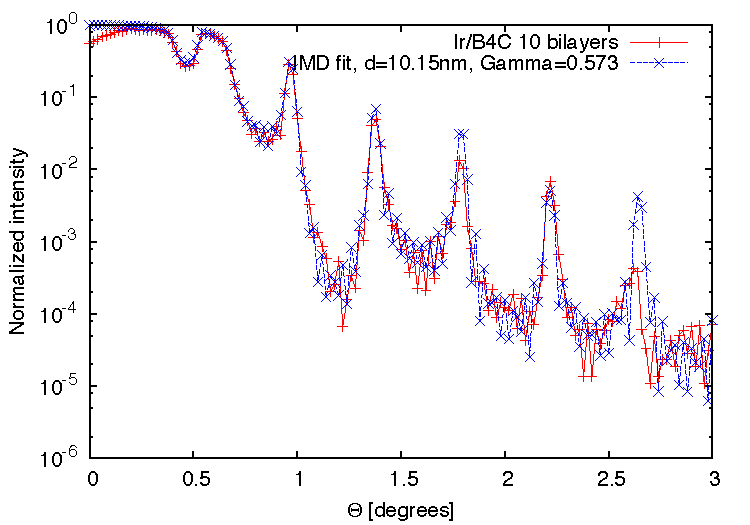
\includegraphics[height=7cm]{figures/chamber/si5811-fit.pdf}
\caption{\footnotesize XRR measurement of a 10 bilayer Ir/B$_4$C coating to calibrate for SPO coating. The measurement is fitted with an IMD model to determine d-spacing $\Gamma$.}\label{fig:irb4c-fit}
\end{figure}

The result for each sample is used to get the specific thickness of a material when coating with a given speed. Each result from the IMD model fitting is put into a table like the following:

%\begin{table}[!h]
\begin{center}
\begin{tabular}{c|c|c|c|c}
Sample & speed (Ir) & speed (B$_4$C) & d-Ir [nm] & d-B$_4$C [nm] \\
\hline
si5809 & 2623 & 473 & 2.42 & 2.54 \\
si5810 & 1445 & 338 & 3.21 & 3.88 \\
si5811 & 1011 & 236 & 4.33 & 5.81 \\
si5812 &  674 & 158 & 6.40 & 8.85 \\
si5813 & 281 & 225 & 14.55 & 7.49
\end{tabular}
\end{center}
%\caption{\footnotesize Calibration samples coated with 10 bilayer Ir/B$_4$C multilayers of different thickness. Each sample is measured using XRR and fitted to an IMD model. \label{tab:AFMsamples}}
%\end{table}

The d-spacings for a given material are plotted as a function of the inverse speed of the sample ring (v$^{-1}$) and fitted with a linear regression as seen in figure \ref{fig:calib-fit}. The $a$ and $b$ values of the linear regression are used directly to determine the speed of the sample ring, $v_{\mathrm{B}_4\mathrm{C}}$, to coat e.g. boron carbide with a thickness of $d_{\mathrm{B}_4\mathrm{C}}$ like so:

\begin{eqnarray}
	v_{\mathrm{B}_4\mathrm{C}} = \frac{a}{d_{\mathrm{B}_4\mathrm{C}}-b}.
\end{eqnarray}

\begin{figure}[!h]
	\center
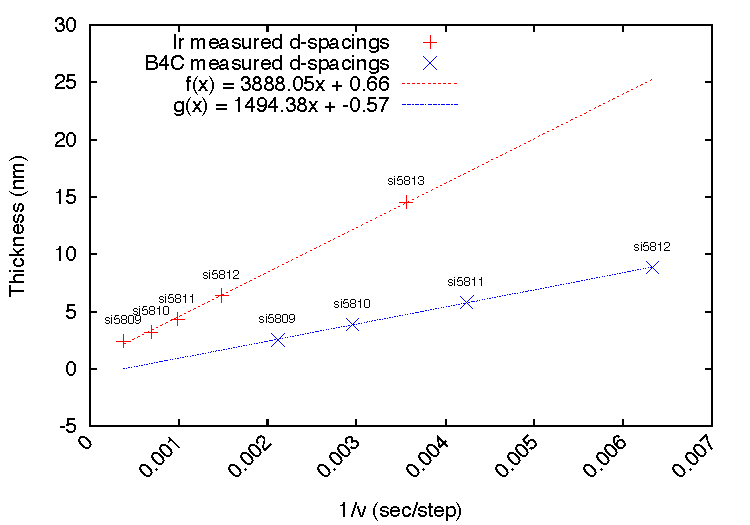
\includegraphics[width=0.8\linewidth]{figures/chamber/calibration_plot-ir-b4c.pdf}
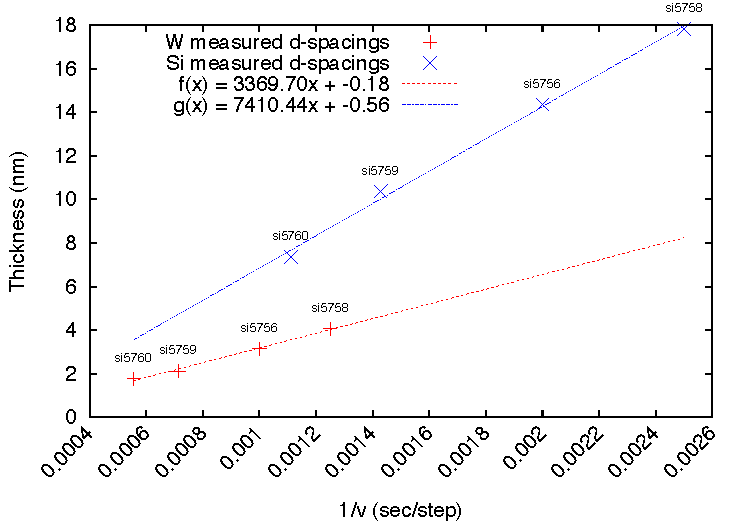
\includegraphics[width=0.8\linewidth]{figures/chamber/calibration_plot-w-si.pdf}
\caption{\footnotesize Linear regression fits of calibration samples for Ir/B$_4$C (top) W/Si (bottom). Each datapoint is the XRR measured thickness of one material layer in a sample.}\label{fig:calib-fit}
\end{figure}
